\subsection{Bestimmung der Verdampfungswärme bei kleinem Druck}
\label{sec:bestimmungverdampfungswarme}
Die Verdampfungswärme kann als Porportionalitätsfaktor zwischen dem natürlichen Logarithmus des Druckes $P$ und der reziproken absoluten Temperatur $T$ aufgefasst werden. Die Wertepaare sind in Tabelle \ref{tab:druck-temperatur} dargestellt.
\begin{figure}
\captionof{table}{Wertepaare für die lineare Regression}	
	\centering
\input{testtabelle(besser).txt}
\label{tab:druck-temperatur}
\end{figure}

\begin{equation}
\ln(P) = - \frac{L}{\text{R}} \frac{1}{T} + \text{const.} = a \cdot \frac{1}{T} +b
\end{equation}
Lineare Regression nach Formeln aus Kapitel (\ref{sec:regression}) mittels Python liefert
\begin{equation}
a= \num{-4910(60)}  \text{Hässliche Einheit hinschreiben?}
\end{equation}
und damit eine Verdampfungswärme des Wassers von
\begin{equation}
L = - a \cdot R = \SI{40800(500)}{\joule\per\mol} 
\end{equation}
wobei $R$ die Gaskonstante mit \SI{8.314}{\joule\per\kelvin\per\mol} ist. \\
.


\begin{figure}[h!]
	\centering
	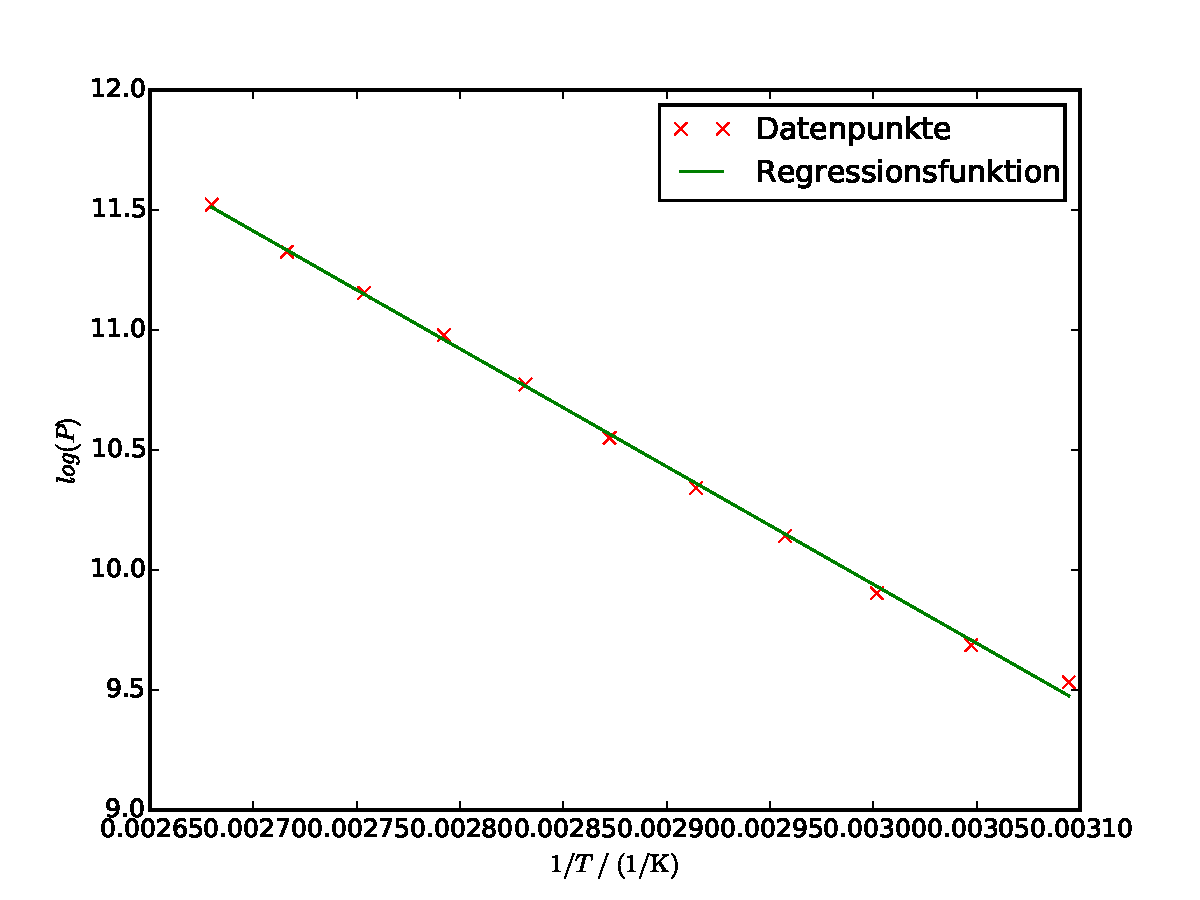
\includegraphics[width=0.95\textwidth]{L_kleiner_Druck.pdf}
	\caption{Logarithmus des Dampfdruckes gegen die reziproke absolute Temperatur}
	\label{fig:L_kleiner_Druck}
\end{figure}

\subsection{Unterscheidung zwischen äußerer und innerer Verdampfungswärme}
Die äußere Verdampfungswärme entspricht der Energie, die von System aufgewendet wird um zu expandieren. Diese Volumenarbeit ist bei einer Temperatur von  \SI{373}{\kelvin}
\begin{equation}
L_\text{a} = p \cdot V_\text{m} = R \cdot T = \SI{8.314}{\joule\per\kelvin\per\mol} \cdot  \SI{373}{\kelvin} \approx \SI{3101}{\joule\per\mol} \quad.
\end{equation}
Die innere Verdampfungswärme wird aufgebracht, um die wechselwirkenden Moleküle voneinander zu trennen. Da in Abschnitt \ref{sec:bestimmungverdampfungswarme} die gesamte Verdampfungswärme bestimmt wurde, entspricht die innere Verdampfungswärme gerade
\begin{equation}
L_\text{i} = L - L_{\text{a}} = \SI{40800}{\joule\per\mol} - \SI{3101}{\joule\per\mol} = \SI{37699}{\joule\per\mol} \quad.
\end{equation}
Die innere Verdampfungswärme ist dominierend. Bei Wasser beträgt der Wert der äußeren Verdampfungswärme unter Normaldruck nur etwa 10 \% des Wertes der Inneren.\cite{TUGraz}
%\footnote{siehe \url{http://portal.tugraz.at/portal/page/portal/Files/i5110/files/Lehre/Praktika/GP1/Vorbereitung/Verdampf_Gesamt.pdf}}




\subsection{Temperaturabhängigkeit der Verdampfungswärme bei hohem Druck}
Die Druck- und Temperaturabhängigkeit der Verdampfungswärme ist nach Formel \eqref{Clausius einfach} mit
\begin{equation}
	L(T, p(T)) = T^2\frac{R}{p}\frac{\text{d}p}{\text{d}T}
\end{equation} gegeben.

Zunächst wird der Druck als Funktion der Temperatur dargestellt. Mit Hilfe von Python wurde für $p(T)$ ein Polynom dritten Grades berechnet. Die hier angegebenen Werte für die Koeffizienten des Polynoms sind gerundet, obwohl mit exakten weiter gerechnet wurde.
\begin{equation}
p(T) = a \cdot T ^3 + b \cdot T^2 +c \cdot T + d
\end{equation}
\begin{align}
a &=0.626 \\
b &= 642 \\
c &= 221564 \\
d  &= 25769772
\end{align}
Die Ableitung des Druckes nach der Zeit ist
\begin{equation}
\frac{\text{d} p}{\text{d} T} = 3 \cdot a \cdot T^2 + 2 \cdot b \cdot T + c
\end{equation}
\begin{figure}[h!]
	\centering
	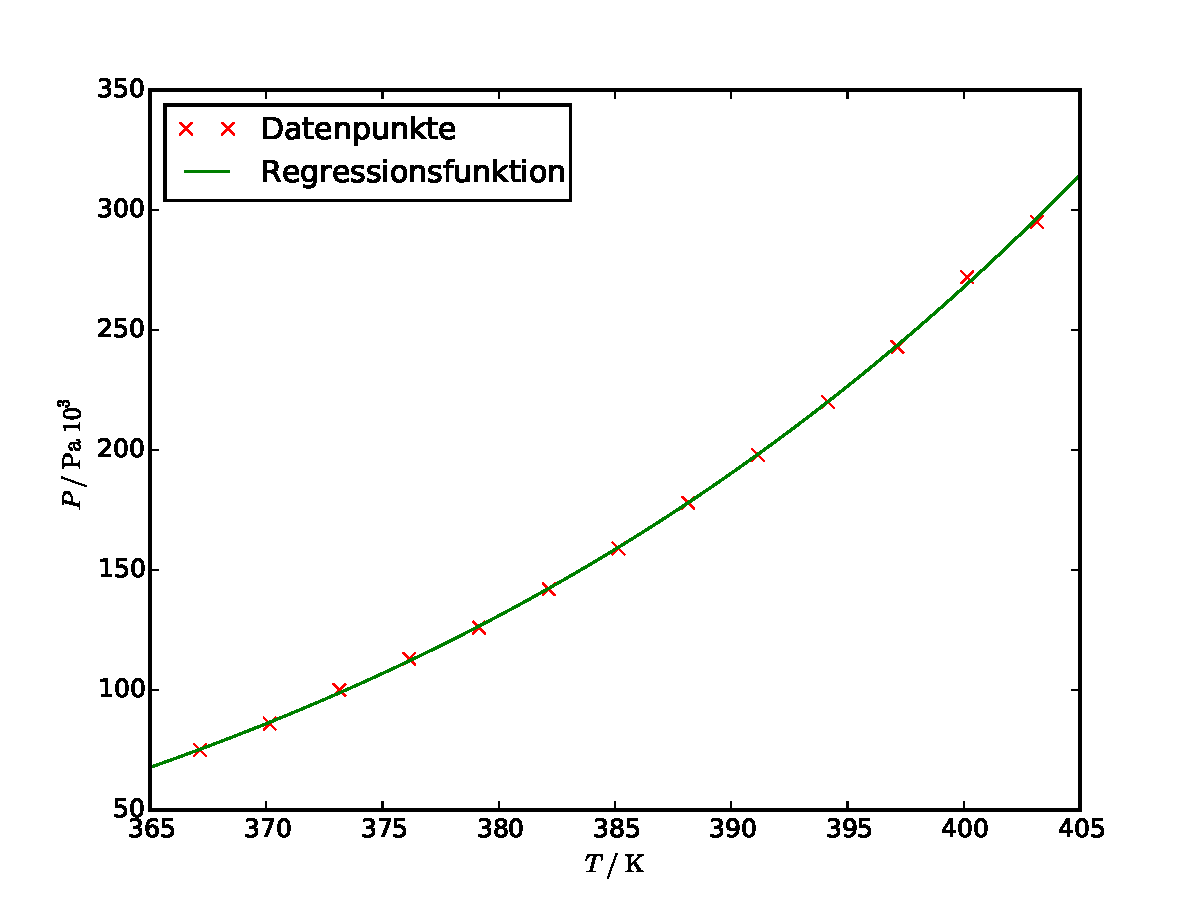
\includegraphics[width=0.95\textwidth]{Regerssionspolynom_P(t).pdf}
	\caption{Regressionspolynom dritten Grades des Druckes über der Temperatur}
	\label{fig:Regerssionspolynom_P(t)}
\end{figure}
\\

Die Volumenabhängigkeit von Temperatur und Druck kann hier nicht mehr vernachlässigt werden. Das ideale Gasgesetz gilt nicht, sodass das Volumen besser durch
\begin{equation}
\left( p(T) + \frac{a_\text{W}}{V^2}\right) = R \cdot T
\end{equation}
\begin{equation}
\Leftrightarrow
V_{+,-}(T, p(T)) = \frac{R \cdot T \pm \sqrt{R^2 \cdot T^2 - 4 \cdot a_\text{W} \cdot p(T)}}{2 \cdot p(T)}
\end{equation}
genähert wird. Durch Einsetzen der Ergebnisse ist ersichtlich, dass die Lösung $V_+$ das reale Volumen wiedergibt. 
Bilder?!
\\
Nach dieser Vorarbeit ist
\begin{equation}
L(T, p(T)) = V_+(T, p(T)) \cdot T \cdot \frac{\text{d} p}{\text{d} T} 
\end{equation}
und wurde in Abbildung \ref{fig:L_groser_druck_temperaturabhangig} über die Temperatur aufgetragen. Zusätzlich wurden die Werte eingetragen, die sich ergeben, wenn die Messwerte von $T$ in $L(T, p(T))$ eingesetzt werden. Die Datenpunkte sind also die $L(T_\text{gemessen})$. 

Wertetabelle?!



\begin{figure}[h!]
	\centering
	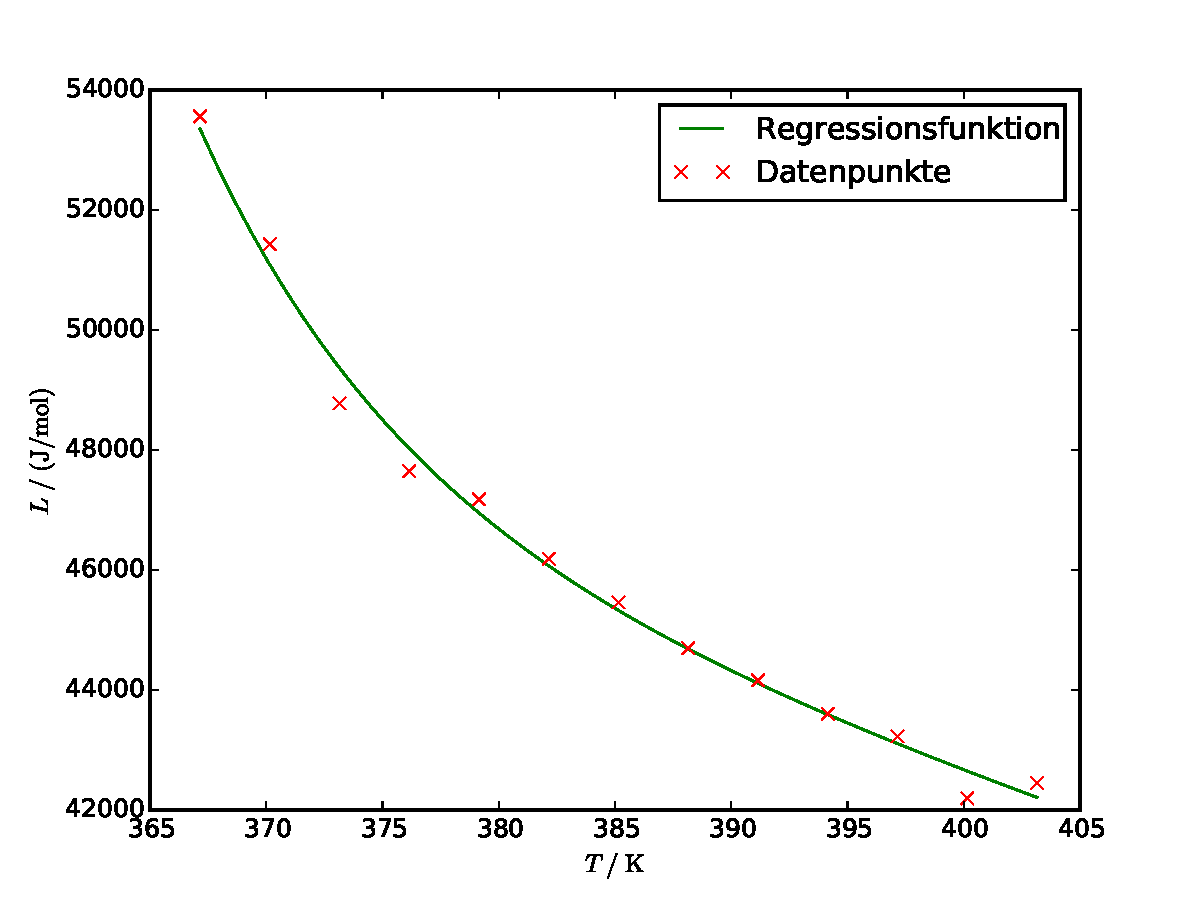
\includegraphics[width=0.95\textwidth]{L_groser_druck_temperaturabhangig.pdf}
	\caption{Verdampfungswärme in Abhängigkeit der Temperatur}
	\label{fig:L_groser_druck_temperaturabhangig}
\end{figure}





